%!TEX ROOT=formularioMatematica.tex

\section{Generale}\label{sec:gen}
In questa sezione verranno trattati alcuni temi utili in tutto il formulario, come i prodotti notevoli
o alcune prprietà dei radicali.\\
Per gli esercizi si vada a pagina~\pageref{ex:generale}.

\subsection{Prodotti notevoli}\label{subsec:gen:prodnot}
I prodotti notevoli sono dei prodotti o delle fattorizzazioni sempre vere per qualunque numero. 
Risultano essere molto utili quando si deve semplificare un'espressione.
\begin{align*}
  a^2 - b^2 &= (a-b)(a+b)\\
  a^3 - b^3 &= (a-b)(a^2+ab+b^2)
\end{align*}
Questi hanno la seguente formula generale
\begin{equation*}
  a^n - b^n = (a-b)(a^{n-1} - a^{n-2}b + a^{n-3}b^2 - \dotsb - ab^{n-2} + b^{n-1})
\end{equation*}
\begin{align*}
  (a\pm b)^2 &= a^2 \pm 2ab + b^2 \\
  (a\pm b)^3 &= a^3 \pm 3a^2b + 3ab^2 \pm b^3
\end{align*}
Questi hanno la seguente formula generale, anche conosciuto come `Binomio di Newton', approfondito
nella sezione dedicata al calcolo combinatorio.
\begin{equation*}
  (a + b)^n = \sum\limits_{k = 0}^{n}\binom{n}{k}a^{n-k}b^k
\end{equation*}

\subsection{Radicali}
I radicali sono delle espressioni spesso irrazionali che contengono almeno una radice. La radice è 
anche pensabile come una potenza
\begin{equation*}
  \sqrt[n]{x^m} = x^{\frac{m}{n}}.
\end{equation*}

\subsubsection{Addizione e Sottrazione}
Due radicali si possono addizionare o sottrarre se e solo se \textbf{sono simili}
\begin{equation*}
  m\cdot\sqrt[n]{a} \pm p\cdot\sqrt[n]{a} = (m\pm p)\cdot\sqrt[n]{a}
\end{equation*}

\subsubsection{Divisione e Moltiplicazione}
Due radicali si possono moltiplicare o dividere se e solo se \textbf{hanno lo stesso indice}
\begin{equation*}
  \sqrt[m]{a}\cdot\sqrt[m]{b} = \sqrt[m]{ab}\qquad\frac{\sqrt[m]{a}}{\sqrt[m]{b}} = \sqrt[m]{\frac{a}{b}}
  ,\quad b \neq 0
\end{equation*}

\subsubsection{Razionalizzare un radicale}
Per razionalizzare un radicale si intende eliminare il radicale dal denominatore di una frazione in
quanto non è possibile dividere un numero per un irrazionale.
\begin{align*}
  \frac{d}{c\cdot\sqrt{b}} & = \frac{d}{c\cdot\sqrt{b}}\cdot\frac{\sqrt{b}}{\sqrt{b}} = 
  \frac{d\cdot\sqrt{b}}{cb} \quad b > 0,\, c \neq 0 \\
  \frac{c}{a\pm\sqrt{b}} &= \frac{c}{a\pm\sqrt{b}}\cdot\frac{a\mp\sqrt{b}}{a\mp\sqrt{b}} = 
  \frac{c\cdot(a\pm\sqrt{b})}{a^2-b} \quad a\pm\sqrt{b} \neq 0 \\
  \frac{c}{\sqrt{a}\pm\sqrt{b}} &=
  \frac{c}{\sqrt{a}\pm\sqrt{b}}\cdot\frac{\sqrt{a}\mp\sqrt{b}}{\sqrt{a}\mp\sqrt{b}} =
  \frac{c(\sqrt{a}\mp\sqrt{b})}{a-b} \quad \sqrt{a}\pm\sqrt{b} \neq 0
\end{align*}
In generale per razionalizzare si deve moltiplicare per un fattore che annulli il radicale stesso, 
generalmente quel fattore è il radicale o il suo reciproco.

\subsubsection{Radicale di un radicale}
Per risolvere o semplificare espressioni come $\sqrt{a\pm\sqrt{b}}$ si può usare questa formula
\begin{equation*}
  \sqrt{a\pm\sqrt{b}} = \sqrt{\frac{a+\sqrt{a^2-b}}{2}}\pm\sqrt{\frac{a-\sqrt{a^2-b}}{2}}
\end{equation*}

\subsubsection{Disequazioni con radicali}
\begin{align*}
  \sqrt{f(x)} > g(x) &\Leftrightarrow \left\{\begin{cases}
      f(x) \geq 0\\
      g(x) < 0
    \end{cases} \cup \begin{cases}
      g(x) \geq 0\\
      f(x) > g^2(x)
  \end{cases}\right\}\\
  \sqrt{f(x)} < g(x) &\Leftrightarrow \begin{cases}
    f(x) \geq 0\\
    g(x) > 0\\
    f(x) < g^2(x)
  \end{cases}\\
  \sqrt{f(x)} \lessgtr \sqrt{g(x)} &\Leftrightarrow \begin{cases}
    f(x) \geq 0\\
    g(x) \geq 0\\
    f(x) \lessgtr g(x)
  \end{cases}
\end{align*}

\subsection{Equazioni particolari}
Ci sono infiniti tipi di equazioni, alcune però hanno delle soluzioni immediate, eccone alcune.

\subsubsection{Equazioni binomie}
Le equazioni binomie sono nella forma $x^n = a$. Le loro soluzioni sono le seguenti
\begin{align*}
  x &= \pm\sqrt[n]{a} &\quad &\text{Se $n$ è pari e $a\geq0$}\\
  x &= \sqrt[n]{a} &\quad &\text{Se $n$ è dispari}
\end{align*}

\subsubsection{Equazioni trinomie e biquadratiche}
Le equazioni trinomie sono nella forma $ax^{2n} + bx^n + c =0$. Se $n=2$ sono definite biquadratiche.\\
Per risolverle si ponga $t = x^n$ e si risolva l'equazione di secondo grado che ne deriva
\begin{equation*}
  at^2 + bt + c = 0
\end{equation*}
e poi si risolva $x^n = y_1$ e $x^n = y_2$.

\subsubsection{Equazioni di secondo grado}
Le equazioni di secondo grado sono tra le più diffuse. Presentano alcune caratteristiche.\\
Sia $ax^2 + bx + c = 0$ la nostra equazione, allora $x_1$ e $x_2$ sono le sue soluzioni. Per trovarle
si usi la seguente formula
\begin{equation*}
  x_{1/2} = \frac{-b\pm\sqrt{b^2-4ac}}{2a}
\end{equation*}
Conoscendo le soluzioni si può semplificare l'equazione in questo modo
\begin{equation*}
  ax^2+bx+c=a(x-x_1)(x-x_2)
\end{equation*}
Vige anche questa particolarità
\begin{equation*}
  x_1+x_2 = -\frac{b}{a} \qquad x_1\cdot x_2 = \frac{c}{a}
\end{equation*}

\subsection{Ruffini}\label{ruffini}
Il metodo di Ruffini permette di ridurre di grado qualsiasi equazione. Prima di usare questo metodo si
dovrebbe però verificare che non sia possibile usare \hyperref[subsec:gen:prodnot]{prodotti notevoli}
in quanto il processo richiede tempo.\\
Per prima cosa si deve trovare uno \textbf{zero} dell'equazione, ovvero una soluzione. Essi sono
da ricercarsi tra le seguenti frazioni
\begin{equation*}
  \text{Zeri} = \frac{\text{Divisori termine noto}}{\text{Divisori $a$}}
\end{equation*}
Per dimostrare l'utilizzo di questa regola, prendiamo come esempio la seguente equazione
\begin{equation}\label{eq:ruffini}
  2x^3 + 3x + 5 = 0
\end{equation}
Lo zero di quest'equazione è $\mathcolor{red}{-1}$, infatti $2\cdot(-1)^3 + 3\cdot(-1) + 5 = 0$. Il 
seguente disegno chiarisce i passaggi da seguire per ridurre di grado un'equazione.
\begin{center}
  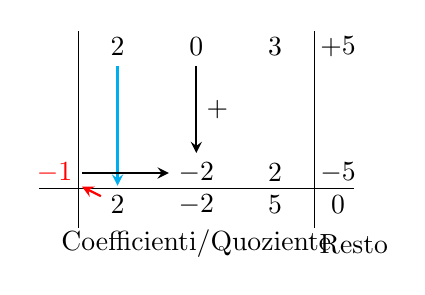
\begin{tikzpicture}
    \draw (-0.5,0) -- (3.5,0);
    \draw (0,2) -- (0,-0.5);
    \draw (3,2) -- (3,-0.5);
    \node[red] (z) at (-0.3,0.2) {$-1$};
    \node (a) at (0.5,1.8) {$2$};
    \node (b) at (1.5,1.8) {$0$};
    \node (c) at (2.5,1.8) {$3$};
    \node (r) at (3.3,1.8) {$+5$};
    \node (b1) at (1.5,0.2) {$-2$};
    \node (c1) at (2.5,0.2) {$2$};
    \node (r1) at (3.3,0.2) {$-5$};
    \node (a2) at (0.5,-0.2) {$2$};
    \node (b2) at (1.5,-0.2) {$-2$};
    \node (c2) at (2.5,-0.2) {$5$};
    \node (r2) at (3.3,-0.2) {$0$};
    \draw[-stealth, thick, cyan] (a) -- (a2);
    \draw[-stealth, thick, red] (a2) -- (z);
    \draw[-stealth, thick] (z) -- (b1);
    \draw[-stealth, thick] (b) -- (b1)
      node[pos=0.5, right]{$+$};
    \node (coef) at (1.5,-0.7) {Coefficienti/Quoziente};
    \node (rest) at (3.5,-0.7) {Resto};
  \end{tikzpicture}
\end{center}

Il processo da seguire è il seguente:
\begin{enumerate}
  \item Moltiplicare il coefficiente del grado massimo per lo zero
  \item Aggiungere al grado successivo il risultato
  \item Continuare fino a che non si arriva al termine noto
\end{enumerate}
Così si otterranno i nuovi coefficienti dell'equazione. Nel nostro caso otteniamo
\begin{equation}\label{eq:ruffini1}
  2x^2 -2x + 5
\end{equation}
però questo non basta in quanto le equazioni~\eqref{eq:ruffini} e~\eqref{eq:ruffini1} non sono 
equivalenti. Per renderle equivalenti, si moltiplichi per $(x-x_0)$ dove $x_0$ è lo zero dell'equazione
originale. Quindi ora abbiamo ottenuto che
\begin{equation*}
  2x^3 + 3x + 5 = (2x^2 -2x + 5)(x+1)
\end{equation*}
E che quindi possiamo dire che $P_n(x) = P_{n-1}(x)\cdot(x-x_0)$ dove $P_n(x)$ è un polinomio di grado
$n$ nella variabile $x$.

% Reset the counter
\setcounter{equation}{0}

\subsection{Regola di Cramer}
La regola di Cramer permette di risolvere sistemi lineari a $n$-incognite. Generalmente non è molto
comodo per grandi valori di $n$ in quanto diventa lungo da risolvere però per due o tre equazioni è
molto comodo.\\ [\baselineskip]
Ogni sistema può essere definito come
\begin{equation*}
  Ax = c
\end{equation*}
dove $A$ è una matrice e $x$ e $c$ sono vettori. Le soluzioni $(x_1,\ldots,x_n)$ sono determinabili
\begin{equation*}
  x_i = \frac{\det A_i}{\det A}
\end{equation*}
dove $A_i$ è la matrice costruita con la $i$-esima colonna di $A$ con il vettore $c$.\\
Esempio a 2 equazioni
\begin{equation*}
  \begin{cases}
    ax+by=\mathcolor{red}{e}\\cx+dy=\mathcolor{red}{f}
  \end{cases} \Leftrightarrow
  \begin{bmatrix}[1]
    a&b\\c&d
  \end{bmatrix}
  \begin{bmatrix}[1]
    x\\y
  \end{bmatrix}=
  \begin{bmatrix}[1]
    \mathcolor{red}{e}\\\mathcolor{red}{f}
  \end{bmatrix}
\end{equation*}
quindi
\begin{align*}
  x = \frac{\begin{vmatrix}[1]
      \mathcolor{red}{e}&b\\\mathcolor{red}{f}&d
    \end{vmatrix}}{\begin{vmatrix}[1]
      a&b\\c&d
  \end{vmatrix}}= \frac{\mathcolor{red}{e}d-b\mathcolor{red}{f}}{ad-bc}
\end{align*}
\begin{align*}
  y = \frac{\begin{vmatrix}[1]
      a&\mathcolor{red}{e}\\c&\mathcolor{red}{f}
    \end{vmatrix}}{\begin{vmatrix}[1]
      a&b\\c&d
  \end{vmatrix}}= \frac{a\mathcolor{red}{f}-\mathcolor{red}{e}c}{ad-bc}
\end{align*}

\subsection{Valori assoluti}
Verranno qui elencate alcune caratteristiche dei valori assoluti.

\subsubsection{Definizione}
\begin{equation*}
  \left\lvert x\right\rvert \Leftrightarrow
  \begin{cases}
    x &\text{se } x \geq 0\\
    -x &\text{se } x < 0
  \end{cases}
\end{equation*}

\subsubsection{Proprietà}
Dalla definizione ne derivano alcune proprietà
\begin{alignat*}{2}
  \left\lvert x\right\rvert &= \left\lvert -x\right\rvert &\qquad 
  \left\lvert x^2\right\rvert&=\left\lvert x\right\rvert^2 = x^2\\
  \left\lvert a+b\right\rvert &\leq \left\lvert a\right\rvert+\left\lvert b\right\rvert & 
  \left\lvert a\cdot b\right\rvert&=\left\lvert a\right\rvert\cdot\left\lvert b\right\rvert
\end{alignat*}

\subsubsection{Funzioni e valori assoluti}
Vengono ora riportati i sistemi risolutivi di funzioni con valori assoluti
\begin{align*}
  \left\lvert f(x)\right\rvert \geq g(x) &\Leftrightarrow 
  \begin{cases}
    f(x) \leq -g(x)\\
    f(x) \geq g(x)
  \end{cases}\\
  \left\lvert f(x)\right\rvert \leq g(x) &\Leftrightarrow -g(x)\leq f(x) \leq g(x)
\end{align*}

\subsection{Geometria}
Qui vengono elencate alcune formule particolari che riguardano la geometria euclidea.

\subsubsection{Teoremi di Euclide}
\begin{center}
  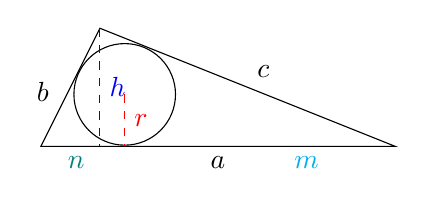
\begin{tikzpicture}[scale=1.5]
    \coordinate (A) at (0.5,1);
    \coordinate (B) at (3,0);
    \coordinate (C) at (0,0);
    \coordinate (O) at (0.71,0.44);


    \draw (A) -- (B) 
      node[pos=0.5, above right]{$c$} -- (C) 
      node[pos=0.5, below]{$a$}
      node[pos=0.25, below, cyan]{$m$}
      node[pos=0.9, below, teal]{$n$} -- cycle 
      node[pos=0.3, above left]{$b$};
    \draw (O) circle (0.43);
    \draw[blue, dashed] (A) -- ++(0,-1)
      node[pos=0.5, right]{$h$};
    \draw[red, dashed] (O) -- ++(0,-0.44)
      node[pos=0.5, right]{$r$};
  \end{tikzpicture}
\end{center}
\begin{alignat*}{2}
  &\textbf{Primo teorema} &\qquad &
  \begin{cases*}
    \dfrac{\mathcolor{cyan}{m}}{c} = \dfrac{c}{a}\\
    \dfrac{\mathcolor{teal}{n}}{b} = \dfrac{b}{a}
  \end{cases*}\\
  &\textbf{Secondo teorema} &\qquad & 
  \frac{\mathcolor{cyan}{m}}{\mathcolor{blue}{h}} = \frac{\mathcolor{blue}{h}}{\mathcolor{teal}{n}}\\
  &\textbf{Proprietà} &\qquad &
  \begin{cases*}
    \mathcolor{blue}{h} = \dfrac{bc}{a}\\
    \mathcolor{red}{r} = \dfrac{b+c-a}{2}
  \end{cases*}
\end{alignat*}

\subsubsection{Formula di Erone}
La formula di Erone permette di trovare l'area di un triangolo qualsiasi conoscendo il semi-perimetro.
\begin{center}
  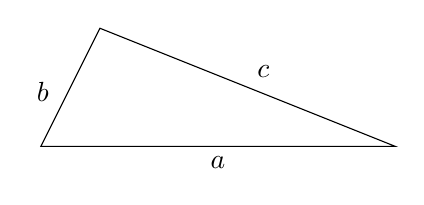
\begin{tikzpicture}[scale=1.5]
    \coordinate (A) at (0.5,1);
    \coordinate (B) at (3,0);
    \coordinate (C) at (0,0);
    \coordinate (O) at (0.71,0.44);

    \draw (A) -- (B) 
      node[pos=0.5, above right]{$c$} -- (C) 
      node[pos=0.5, below]{$a$} -- cycle 
      node[pos=0.3, above left]{$b$};
  \end{tikzpicture}
\end{center}
\begin{equation*}
  S = \sqrt{p(p-a)(p-b)(p-c)}
\end{equation*}

\subsubsection{Raggio di una circonferenza inscritta di un triangolo}
\begin{equation*}
  r = \frac{\mathscr{A}}{p}
\end{equation*}

\subsubsection{Raggio di una circonferenza circosccritta di un triangolo}
\begin{equation*}
  R = \frac{a}{2\sin\alpha} = \frac{abc}{4\mathscr{A}}
\end{equation*}
